\chapter{Contributions} \label{chap:Contributions}


\section*{Introduction}
With the birth of the smart grid as the next step of evolution for grid infrastructure, with the improvements that the smart grid came with, like improved reliability, automation, and faster detection and response to failures, it also came with its own set of risks and disadvantages. mainly due to the fact that it is composed of multiple components and systems that are connected to the internet, like wireless networks and sensors, smart meters, and IoT devices, making it an easy target for hackers. independent groups or state actors whose goal is to cause as much damage as possible or to collect valuable data. On top of those components, there are legacy systems that the smart grid relies on that are known for their many and major security vulnerabilities, which are all easy targets, for example, Supervisory Control and Data Acquisition (SCADA). As an example of those risks and weaknesses, we can look at the situation Ukraine found itself in after Russia targeted their smart grid systems in 2015, leaving 80,000 Ukrainian households without power for 3 to 6 hours. \cite{ukrain-sg-attack}.

That's why it is important to protect the smart grid system from cyberattacks by employing IDS, IPS, and IDPS. 
as the second line of defense in case encryption and authorization were unsuccessful in stopping the cyberattack from targeting the smart grid system.

\newpage




\section{intrusion detection systems (IDS)}
An intrusion detection system is a piece of hardware or software that is responsible for detecting suspicious and malicious activity, and in a network or an information system, the anomaly can either be reported to a systems administrator or saved to a security information and even management system (SIEM), the SIEM combines the output from multiple sources, then uses some filtering techniques to decide if the reported activity is malicious. \cite{1}






\section{intrusion detection systems architecture}
%file:///C:/Users/doo/Desktop/thesis/Securing%20the%20Smart%20Grid%20A%20Comprehensive%20Compilation%20of%20Intrusion%20Detection%20and%20Prevention%20Systems%20(PANAGIOTIS%20I.%20RADOGLOU-GRAMMATIKIS%20etc.).pdf
page 6

\section{intrusion detection systems classification}

Intrusion detection systems are categorized into 2 categories based on the location of the detection, which are either network or host-based (HIDS or NIDS), There are also two primary methods of intrusion detection: signature-based and anomaly-based. \cite{2}

https://onlinelibrary.wiley.com/doi/10.1002/ett.4150


\subsection{Categories}






\subsubsection{NIDS}
Network intrusion detection systems are placed at the point closest to the start of the sub-network right after the firewall so it can have access to all inbound traffic to all devices on the network 



\begin{figure}[h]
	\centering
	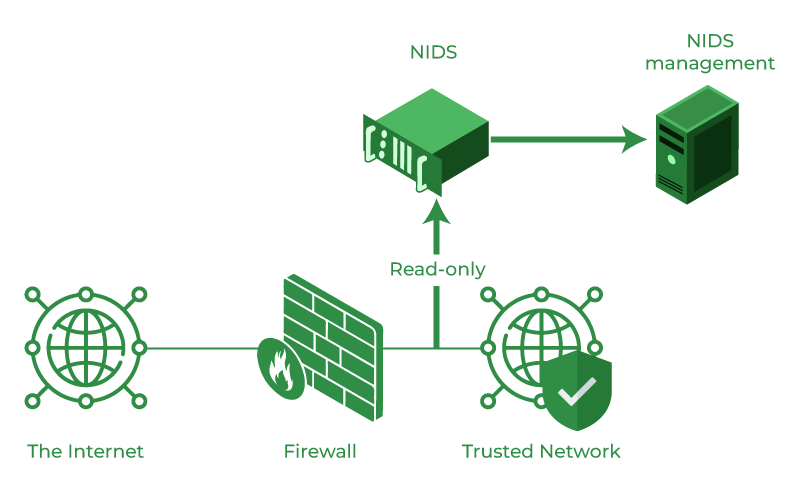
\includegraphics[width=300px]{figures/NIDS.png}
	\caption{NIDS \cite{HIDS-and-NIDS-geeksforgeeks}}
	\label{fig:NIDS}
\end{figure}



\subsubsection{HIDS}
HIDS are placed in indevedule devices in a network and it monitors all incoming and outgoing traffic

\begin{figure}[h]
	\centering
	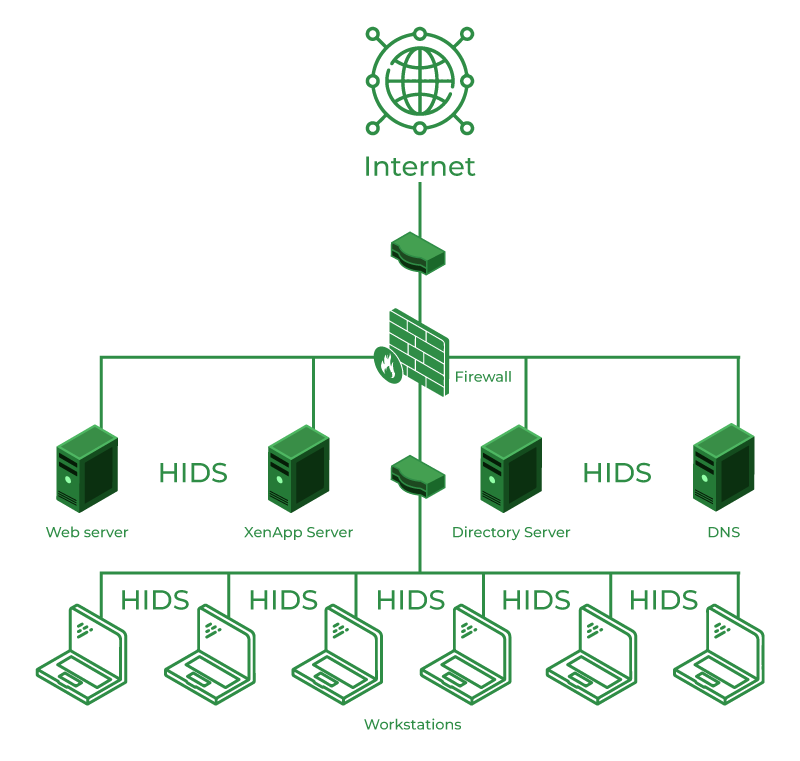
\includegraphics[width=300px]{figures/HIDS.png}
	\caption{HIDS \cite{HIDS-and-NIDS-geeksforgeeks}}
	\label{fig:HIDS}
\end{figure}



\subsubsection{PIDS}
\subsubsection{APIDS}
\subsubsection{Hybrid IDS}




\subsection{Detection methods}
\subsubsection{anomaly-based IDS}
\subsubsection{signature-based IDS}
\subsubsection{hybrid IDS}
is in development



\section{maybe IDS vs IPS + IDPS}

\section{maybe IDS usage in smart grid}


\section{conclusion}













\chapter{Implementation} \label{chap:Implementation}
